\include{extsize}
\documentclass[19.9pt]{beamer}
\usepackage{listings}
\usetheme{Singapore}
%\setbeamerfont{frametitle}{size=\normalsize}
%\setbeamerfont{title}{size=\normalsize}
%\useoutertheme{}
\newcommand{\txtonimg}[1]{
\begin{center}
 \fcolorbox{red}{black}{
 \textcolor{white}
 {#1}
 }
 \end{center}
 }
\newcommand{\img}[1]{
			\begin{center}
				\includegraphics[height=6cm]{images/#1}
			\end{center}		
}
\newcommand{\imgslide}[2]{
		{\setbeamertemplate{background canvas}{
		\includegraphics [width=\paperwidth,height=\paperheight]{images/#1}} 
			\begin{frame}[plain]
				\txtonimg{#2}
			\end{frame}
		}
}
\newcommand{\pycode}[1]{
			\lstset{language=python}			
				 \lstinputlisting{code/#1}
}
\newcommand{\htmlcodesm}[1]{
			\lstset{language=html}
				\small			
				 \lstinputlisting{code/#1}
}
\newcommand{\pycodesm}[1]{
			\small
			\pycode{#1}
}
\newcommand{\pycodetiny}[1]{
			\tiny
			\pycode{#1}
}

\title{Building Pluggable Web Applications using
}
\institute{Agiliq Solutions}
\subtitle{
\includegraphics[height=1cm]{images/django.png}}
\author{Lakshman Prasad}
\date{
	
\includegraphics[height=1cm]{images/GIDS_Logo.jpg}\linebreak
	April 21, 2010}

\begin{document}

\begin{frame}
	\titlepage
\end{frame}

\section{Introduction}
	\subsection{Definition}
		\begin{frame}
			{
\includegraphics[height=1cm]{images/django.png}\linebreak
				
\includegraphics[height=1cm]{images/python-logo.png}}
		\begin{itemize}                                                 				\item
			For building \alert{database driven} web applications                 \pause \item
			Emphasis on Reuse, DRY and simplicity
		\end{itemize}
		\end{frame}
	\subsection{A Case Study: Youtube Stars}
		\begin{frame}
			{Hypothetical Application}
			\begin{center}
				
\includegraphics[height=1cm]{images/python-logo.png}
			\end{center}		
		\end{frame}
		\begin{frame}[fragile]
			{Install a pluggable app \alert{django-star-rating} }
			\begin{verbatim}			
			$pip install django-star-rating
			\end{verbatim}
			\lstset{language=python}			
				 \lstinputlisting{code/settings.py}
		\end{frame}
		\begin{frame}
			{Point to an url pattern}
			\lstset{language=python}			
				 \lstinputlisting{code/urls.py}
		\end{frame}
		\begin{frame}
			{Put the template where you want!}
			\lstset{language=html}			
				 \lstinputlisting{code/template.html}			
		\end{frame}
	\begin{frame}
	  \tableofcontents
	 \end{frame}
	\subsection{Overview}
		\begin{frame}
			{Developed at Lawrence-Journal World}
			\img{core_devs.jpg}
		\end{frame}

		\imgslide{exponential.jpg}{~5 million hits per month}

		{\setbeamertemplate{background canvas}{
			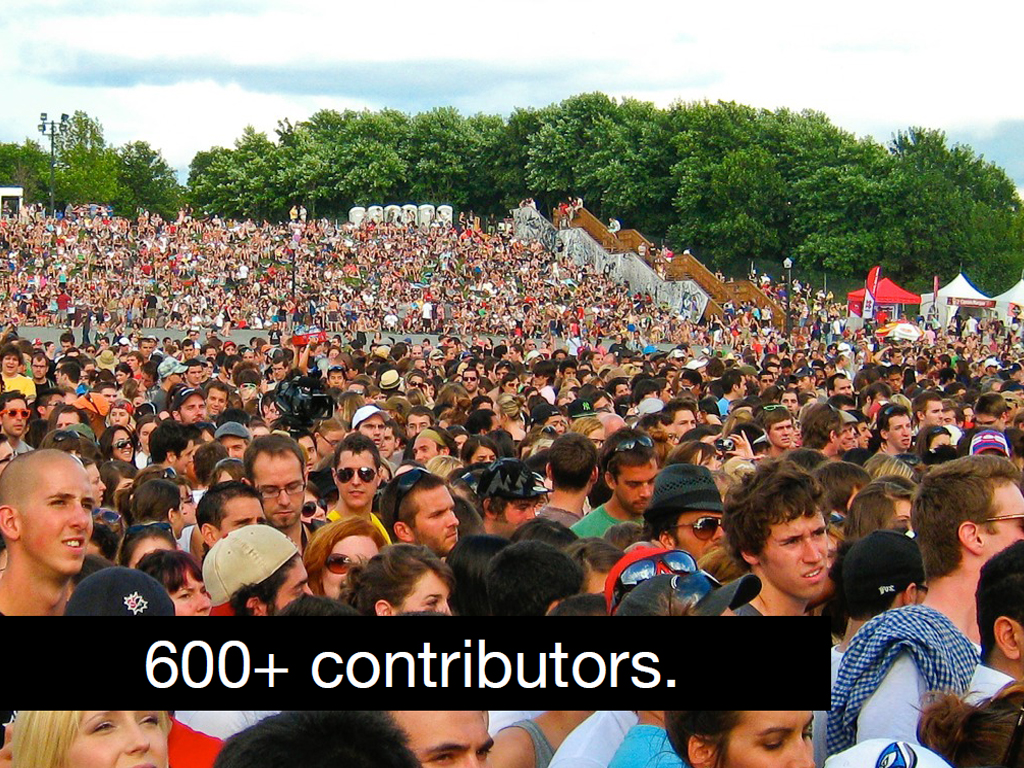
\includegraphics [width=\paperwidth,height=\paperheight]{images/600-contributors.jpg}} 
			\begin{frame}[plain]
			\end{frame}
		}
		
		\imgslide{5-years.jpg}{~5 years since Open Source}
		
	\subsection{Philosophy}		
		\begin{frame}
			{Philosophy}
			\img{philosophy.jpg}
		\end{frame}
		\imgslide{repeat.jpg}{Automate repetitive tasks}
		\imgslide{make-development-fast.jpg}{Make Development Fast}
		\begin{frame}
			{Convention Over Configuration}
			\img{convention.jpg}
		\end{frame}
	
\section{Using django}
	\subsection{MTV}
		\imgslide{models.jpg}{Models}
		\begin{frame}
			{Model Syntax}
			\pycodesm{models.py}
		\end{frame}
		\begin{frame}
			{Admin by models alone}
			\img{admin.png}
		\end{frame}
		\begin{frame}
			{Ugly urls}
			\pycode{uglyurl.txt}
		\end{frame}
		\begin{frame}
			{Good urls}
			\pycode{goodurl.txt}
		\end{frame}
		\begin{frame}
			{django url pattern}
			\pycode{urls.py}
		\end{frame}
		\imgslide{antenna.jpg}{Views}
		\begin{frame}
			{django views}
			\pycodesm{views.py}
		\end{frame}
		\imgslide{template.jpg}{Templates}
		\begin{frame}
			{django template}
			\htmlcodesm{index.html}
		\end{frame}



\section{Features of django}
	\subsection{Features}
		\imgslide{swiss-army-knife.jpg}{Features}
		\begin{frame}
		\begin{itemize}[<+-| alert@+>]                  \item
			Admin Interface                         \item
			Generic Views                           \item
			Testing Tools                           \item
			Sessions                                \item
			Authentication                          \item
			Caching                                 \item
			Internationalization                    \item
			RSS                                     \item
			CSRF protection                         \item
			File Storage                            
		\end{itemize}
		\end{frame}
		\imgslide{docs.png}{Django Documentation}

\section{Reuseable apps}
	\subsection{Writing reuseable apps}
		\begin{frame}
			General conventions adopted by the community
		\end{frame}
		\begin{frame}[<+-| alert@+>]
			{High Level}                                        
		\begin{itemize}                                                    \item
			Use template tags                                              \item
			Use signals                             
		\end{itemize}
		\end{frame}
		\begin{frame}[fragile]
			{Basics}                                                       
		\begin{itemize}[<+-| alert@+>]                                                    \item
			Take \verb|template_name| and \verb|extra_context| every where          \item
			Write urls in applications                                             \item
			Import from the application level                        \item
			Prefix template name with directory                      \item
			Use \verb|MEDIA_URL| in templates                        \item
			Reverse url patterns
		\end{itemize}
		\end{frame}
		\begin{frame}
			{Advanced}                              
		\begin{itemize}[<+-| alert@+>]                                                 
			\item
			Use Template Response                                           
			 \item
			Write Views as Classes
		\end{itemize}
		\end{frame}
		
	\subsection{Community Applications}
		\imgslide{apps.png}{There is an app for that}
		\imgslide{choices.jpg}{For every size and style}
		\begin{frame}
			{Github Search "django"}
			~3000 repositories!
		\end{frame}
		\begin{frame}
			{Pinax}
			\img{pinax2.png}
		\end{frame}
		\begin{frame}
			{django-mingus}
			\pycodesm{mingus.py}
		\end{frame}

\section{End Notes}
	\subsection{Django Stats}
		\begin{frame}
			{Django users}
		\end{frame}
		\begin{frame}
		{Popular Users}
		\begin{itemize}[<+-| alert@+>]
		 \item                                                 
			Media
			\begin{itemize}
			    \item 
				LA Times
				\item
				NY Times
				 \item
				Washington Post
				 \item
				Guardian.
			\end{itemize}
		 \item
			Web2.0
			\begin{itemize}            
				\item 
				Mahalo: 10 million Page views            
				\item
				Pownce
			\end{itemize}
		\item
			Full List: djangosites.com
		\end{itemize}
		\end{frame}
		\begin{frame}
			{NASA}
			\begin{quotation}
			After an extensive trade study, we selected Django as the first and primary application environment for the Nebula Cloud.
			\end{quotation} 
		\end{frame}
	\subsection{Common Enterprise Hurdles}
		\begin{frame}
			{Multiple Databases}
		\end{frame}
		\begin{frame}
			{Dynamic settings infrastructure}
		\end{frame}
		\begin{frame}
			{Tools}
		\end{frame}
	
	
	\subsection{Other}
		\begin{frame}
			{About Me}
		\end{frame}
		\begin{frame}
			{Image Attributions}
		\end{frame}
		\begin{frame}
			?
		\end{frame}




\end{document}
